% \vspace{-0.6in}
\vspace{-0.07in}
\section{Experiments}
\label{sec:experiments}

\begin{figure}[t]
\vspace{-0.4in}
    \centering
    \begin{subfigure}[t]{0.326\linewidth}
        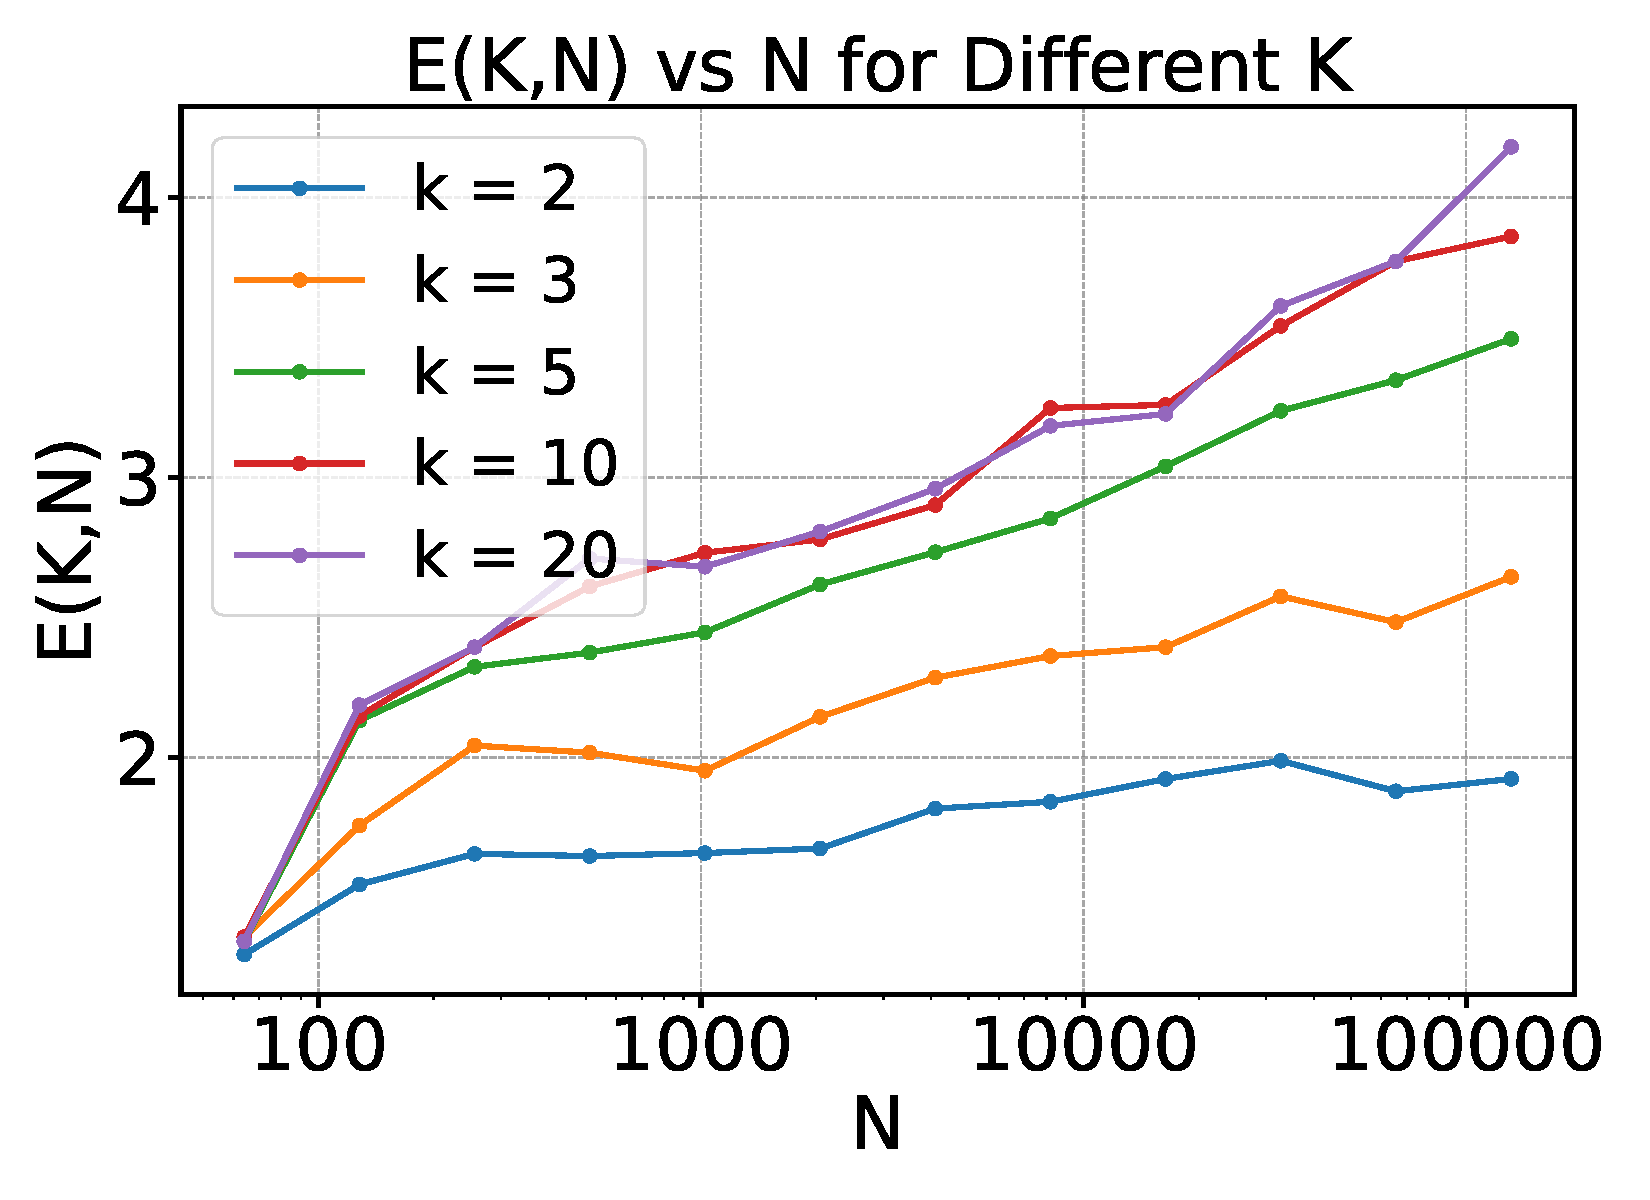
\includegraphics[width=\linewidth]{figs/E_k_avg_vs_N_log_wide_bold.pdf}
        \caption{Strongly convex case: $E(K,N)$ with $N$.}
        \label{fig:strongly-convex-EK-for-N}
    \end{subfigure}
    \begin{subfigure}[t]{0.634\linewidth}
        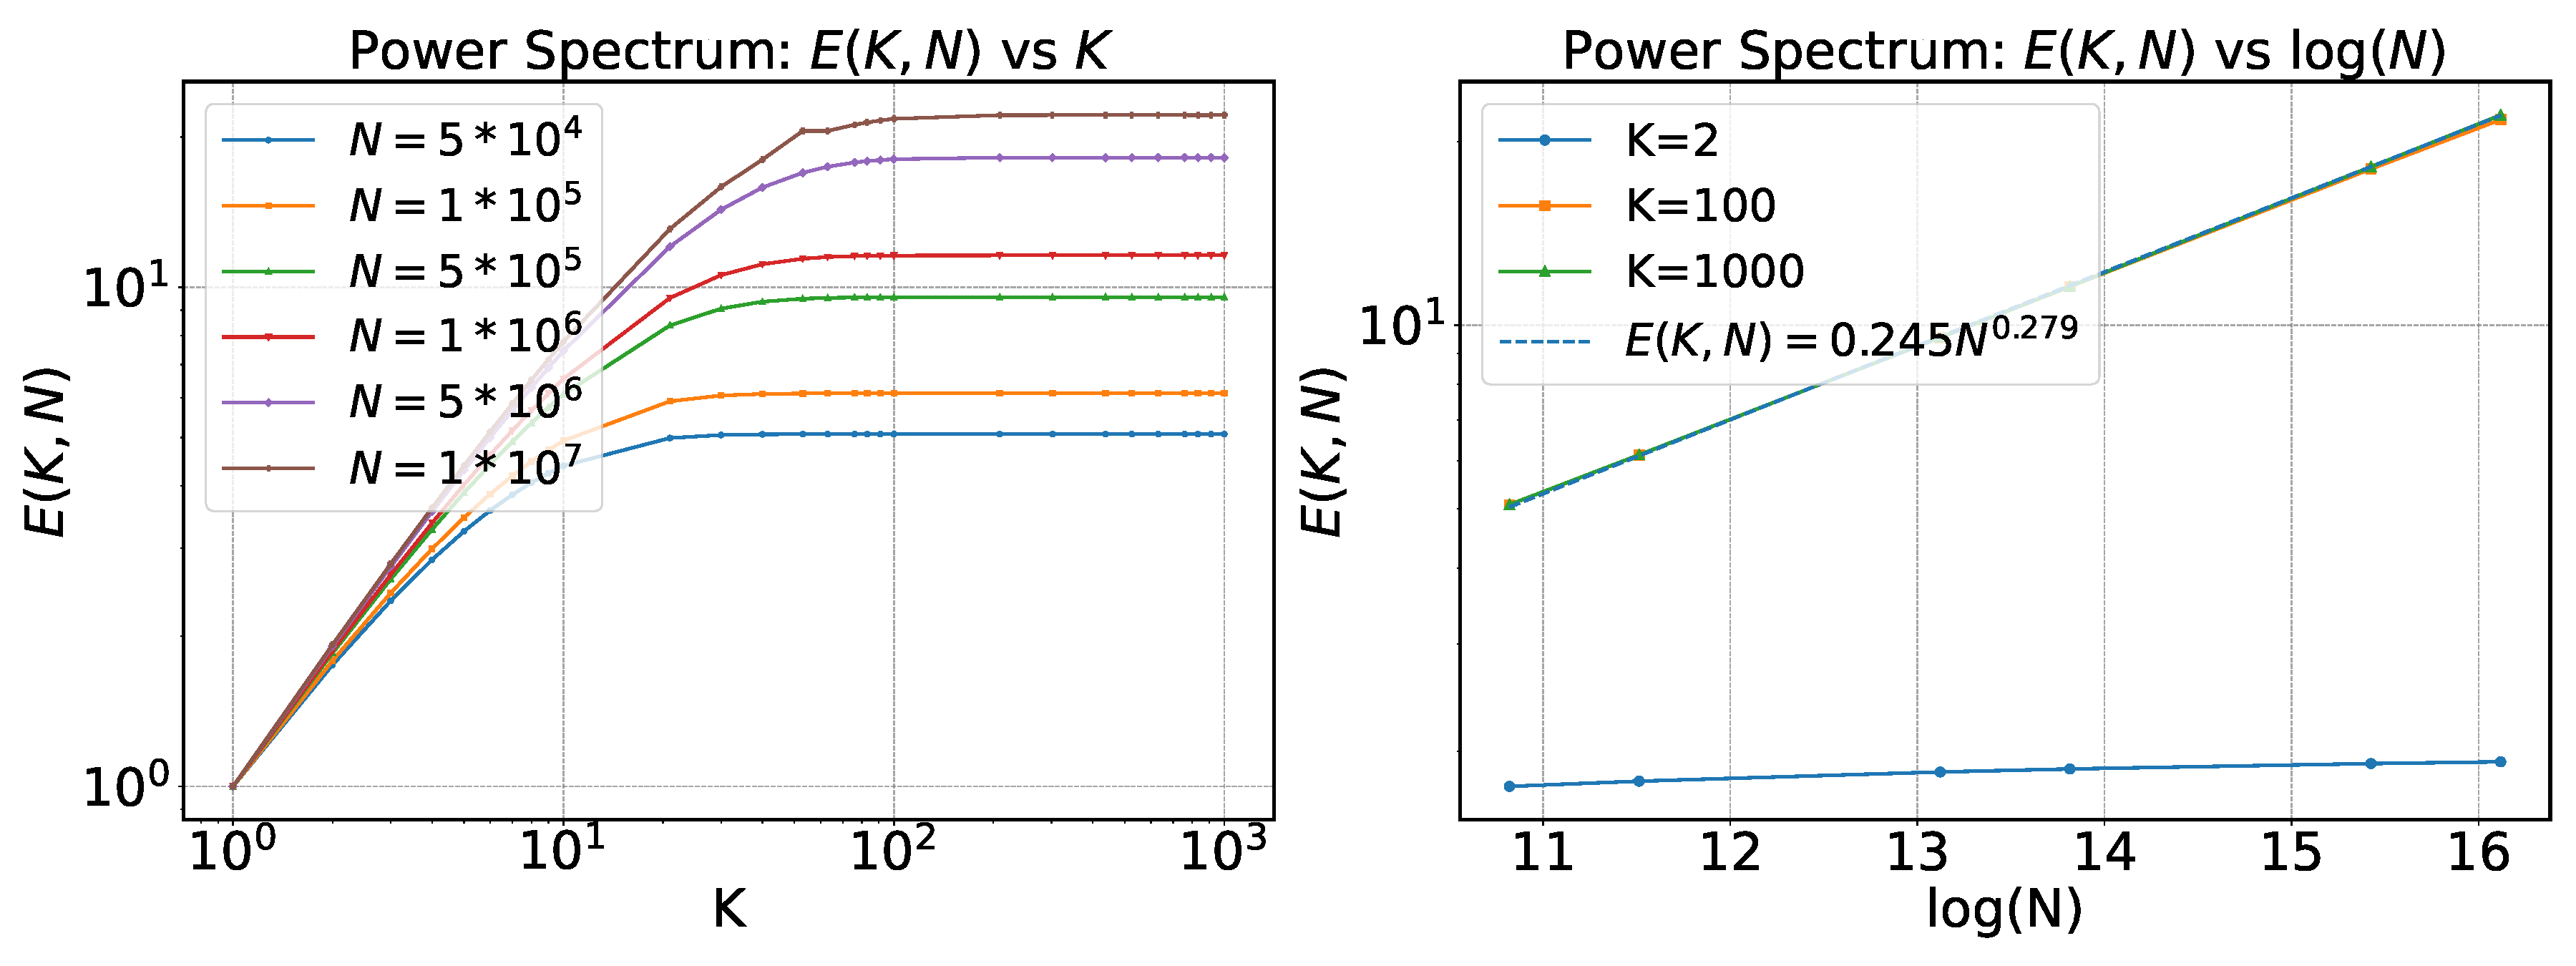
\includegraphics[width=\linewidth]{figs/E_K_comparison_power.pdf}
        \caption{\small The solvable case with Zipf-distributed data and power spectrum: $E(K,N)$ versus $K$ and $N$.}
        \label{fig:one-hot}
    \end{subfigure}
    \caption{\small Simulation experiments for strongly-convex linear regression and the solvable case with Zipf-distributed data and power spectrum. Results show that $E(K,N)$ is approximately proportional to some function of $N$ when $N$ is relatively small, and $E(K,N)\approx K$ when $N$ is relatively large. For the solvable case with Zipf-distributed data and power spectrum, we also fit the effective reuse rate using the formula $E(K,N)=c_1N^{c_2}$ suggested by \Cref{thm:one-hot-E_K-v2}, and the fitted exponent $c_2=0.279\approx\frac{b}{a-b}=\frac{2}{7}$ matches our theory.}
    % \haodong{rewrite the caption, reorganize the subfigures; replot the firgure (a), plot from $N=64$}
    % \tingkai{strongly-convex + power, put log into the appendix; delete the grid in strongly convex case}
% \vspace{-0.25in}
    \label{fig:convex-and-power}
\end{figure} 

%\subsection{Numerical Simulation in Synthetic Datasets}
%Now we validate our theory with experiments on synthetic data under two settings: one corresponding to the strongly-convex scenario of \Cref{sec:strongly_convex}, and another using the solvable model of \Cref{sec:one_hot}. 
\vspace{-0.3cm}
\subsection{Simulations in \Cref{sec:strongly_convex}}
% \vspace{-0.3cm}
% \tingkai{add section 5: power. add log into appendix.}

First, we conduct our experiments on synthetic datasets with a strongly convex linear regression to verify the characterization of effective reuse rate $E(K,N)$ in \Cref{thm:convex-E_K}.
% \kaifengclaw{Typo: 'on synthetic dataset' -> 'on a synthetic dataset' or 'on synthetic datasets'.} 

\paragraph{Experiments Setup.}  We generate data pairs $(\vx_i,y_i)$ where $\vx_i \overset{i.i.d}{\sim}\gN(0,\mI_d)$ with dimension $d = 100$. For the label $y_i$, we generate it as $y_i = \inp{\vw^*}{\vx_i} + \xi_i$, where $\vw^*$ is the ground truth generated by standard Gaussian with unit variance.
% \kaifengclaw{Typo: 'generate' -> 'generated'; 'Gaussin' -> 'Gaussian'.} 
Also, $\xi_i\overset{i.i.d}{\sim}\gN(0,\sigma^2\mI_d)$. Here in our simulation, we set $\sigma$ to $0.1$. To make our simulation aligned with the theoretical setup, we set the learning rate $\eta \propto \frac{\log KN}{KN}$, and we grid search the ratio $c:=\frac{\eta}{\log KN/KN}$ for the $c^*$ which minimizes the final loss given training steps $T=KN$. 

\paragraph{Results.} As shown in \Cref{fig:strongly-convex-EK-for-N}, we plot $E(K,N)$ as a function of $\log N$ for various fixed values of $K$. Each curve corresponds to a fixed number of epochs (e.g., $K=3,5,\dots,20$) and illustrates how the effective reuse rate $E(K,N)$ grows with dataset size. For small data size ($\log N \ll K$), the effective reuse factor increases roughly linearly with $\log N$, indicating that adding more data substantially boosts the one-pass equivalent performance. However, as $N$ becomes large ($\log N \gg K$), each curve flattens out and approaches an asymptote at $E(K,N)\approx K$. In other words, once the dataset is sufficiently large relative to the number of epochs, additional passes through the same data yield no further benefit beyond a factor of $K$. This behavior is exactly as predicted by \Cref{thm:convex-E_K}: when $K$ is much smaller than $\log N$, we have $E(K,N)\approx K$ (nearly full $K$-fold data reuse), whereas when $K$ is large relative to $\log N$, the effective reuse saturates and grows only on the order of $\log N$.

% \vspace*{-0.8cm}
\vspace{-0.4cm}
\subsection{Simulations in \Cref{sec:power-spectrum}} \label{sec:power-spectrum-experiment}
\vspace{-0.3cm}
We now verify the predictions of \Cref{thm:one-hot-E_K-v2} using synthetic data generated under the spectral assumptions of \Cref{sec:one_hot} 
% Because \Cref{thm:one-hot-loss-estimate} provides a closed-form expression for the multi-epoch loss in these settings, we can perform a more controlled simulation of $E(K,N)$. 
% In particular, we consider two cases: (i) 
with a power-law decay Hessian spectrum (\Cref{asp:prior-probability-and-norm}).
% , and (ii) a log-power decay spectrum (\Cref{asp:log-power-decay-prior}), corresponding to the conditions of \Cref{thm:one-hot-E_K-v2} and \Cref{thm:one-hot-E_K-log-spectrum}, respectively.
% \paragraph{Experiments Setup.} 
In all sub-figures of \Cref{fig:one-hot}, we set the data dimension $d$ to $10^5$ and tune all the learning rates to their optimal values. Here we set $a=4.5$ and $b=1$.
% \kaifengclaw{Possible typo: this sentence seems incomplete (likely intended '$a=4.5$ and $b=1$').} 

% . Additionally, we separately tune the spectrum parameters $a$ and $b$ in each sub-figure of \Cref{fig:one-hot}. Specifically, in the top-left and top-right panels, we set $a=4.5$ and $b=1$, whereas in the bottom-left and bottom-right panels, we set $a=1.5$ and $b=2$. 
% In the simulations of the power spectrum case, we 
% \paragraph{Simulations in Power Spectrum Case.} 
% The top-left panel of \Cref{fig:one-hot} plots $E(K,N)$ versus $\log K$ for various fixed $N$, while the right panels show $E(K,N)$ versus $\log N$ for various fixed $K$. In the power-law spectrum scenario, we observe an initial regime where $E(K,N)$ increases almost linearly with $K$ (indicating that more epochs initially provide almost proportional gains in effective data usage), followed by a clear saturation regime where $E(K,N)$ approaches a constant plateau even as $K$ continues to grow. This plateau value is much lower than $K$ when $K$ is large, and it depends on $N$ in a manner consistent with our theory. Specifically, $E(K,N)$ eventually saturates at an asymptotic value, and larger datasets yield higher saturation levels, reflecting a dataset-dependent multiple-epoch benefit, as predicted by \Cref{thm:one-hot-E_K-v2}.  

% % \begin{figure}[htbp]
% % \begin{figure}[t!]
% %     \centering
% %     \includegraphics[width=0.6\linewidth]{figures/one-hot-simulation/E_K_comparison_2x2_paper.pdf}
% %     \caption{Simulation results in the solvable case with power law. \textbf{Top-Left:}}
% %     \label{fig:one-hot}
% % \end{figure}

% \paragraph{Simulations in Log-Power Spectrum Case.} 
% In the log-power spectrum setting (bottom panels of \Cref{fig:one-hot}), $E(K,N)$ exhibits a similar two-regime behavior: the initial growth with $K$ transitions to a plateau whose height increases only logarithmically with $N$ (on the order of $\log^b N$), as described by \Cref{thm:one-hot-E_K-log-spectrum}. The curves depicting $E(K,N)$ versus $\log N$ further illustrate that, for fixed small values of $K$, increasing $N$ eventually yields diminishing returns as $E(K,N)$ approaches the $K$ limit (analogous to the strongly-convex case). For larger values of $K$, however, the effective multiplier reaches a ceiling determined by the dataset-dependent saturation value. These experiments demonstrate the anticipated saturation effects, multiple scaling regimes, and asymptotic plateaus, providing empirical confirmation of the scaling behaviors predicted by \Cref{thm:one-hot-E_K-v2} and \Cref{thm:one-hot-E_K-log-spectrum}.

\paragraph{Results.} \Cref{fig:one-hot} plots $E(K, N)$ versus $K$ and $\log N$ for the solvable model with Zipf-distributed  data. The curves depicting $E(K,N)$ versus $K$ show that $E(K,N)\approx K$ when $K$ is relatively small and saturate to some value depending on $N$ when $K$ is large. In the right panel, which describes the relationship between $E(K,N)$ and $\log N$, we observe that when $K$ is small (namely $K=2$), $E(K,N)$ increases and approaches $K$ as $\log N$ increases, and the plots overlap when $K$ is large. Those phenomena provide empirical confirmation of the scaling behaviors predicted by \Cref{thm:one-hot-E_K-v2}. We also fit $E(K,N)$ in the large-$K$ regime with a power-form function as stated in \Cref{thm:one-hot-E_K-v2}. The fitted exponent is $0.279 \approx \tfrac{b}{a-b} = \tfrac{2}{7}$, aligning with our theory.
% \begin{figure}[t]
% \vspace{-0.5in}
%     \centering
%     \includegraphics[width=0.5\linewidth]{figures/strongly-convex/E_k_avg_vs_N_log_wide_bold.pdf}
%     \caption{Strongly convex case: $E(K,N)$ with $N$}
%     \label{fig:strongly-convex-EK-for-N}
% \vspace{-0.25in}
% \end{figure}

% \begin{figure}[t]
% % \vspace{-0.6in}
%     \centering
%     \begin{subfigure}[b]{0.48\linewidth}
%         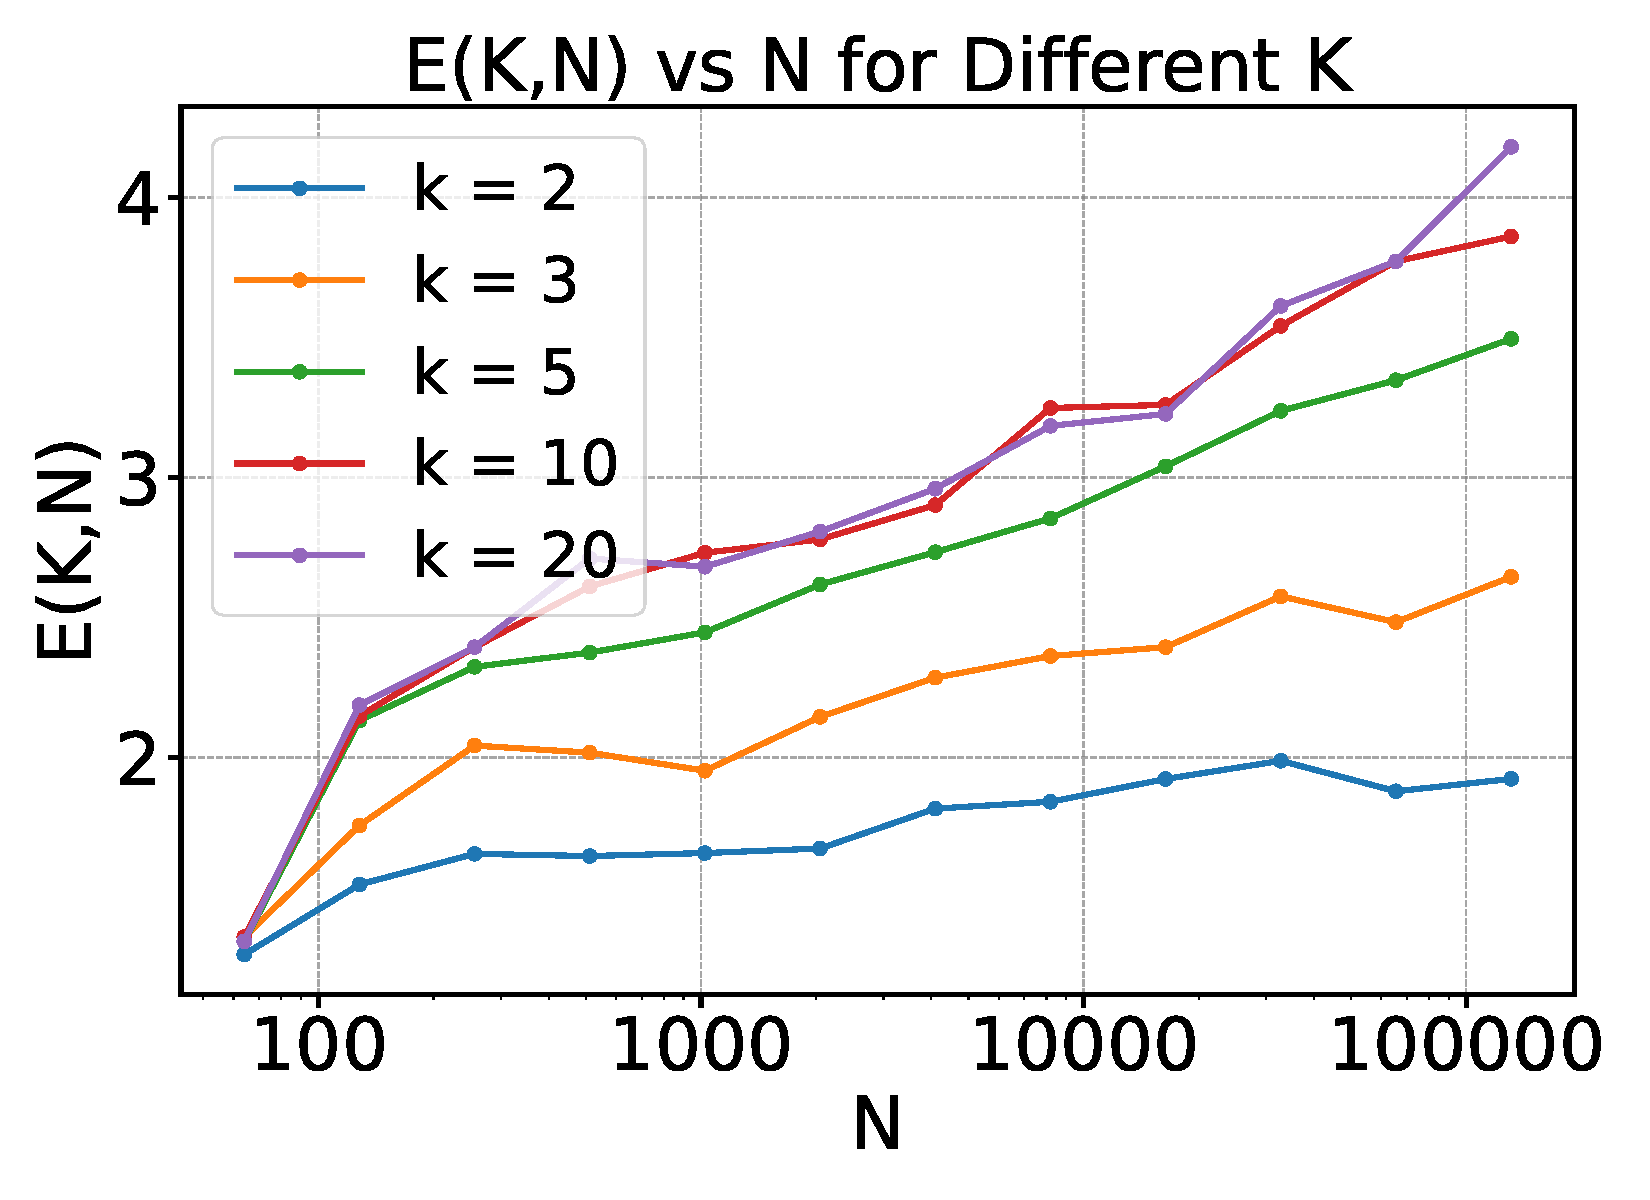
\includegraphics[width=\linewidth]{figs/E_k_avg_vs_N_log_wide_bold.pdf}
%         \caption{Strongly convex case: $E(K,N)$ with $N$}
%         \label{fig:strongly-convex-EK-for-N}
%     \end{subfigure}
%     \begin{subfigure}[b]{0.48\linewidth}
%         \includegraphics[width=\linewidth]{figs/E_K_comparison_2x2_paper.pdf}
%         \caption{The solvable cases with power law in simulation.}
%         \label{fig:one-hot}
%     \end{subfigure}
%     \caption{Simulation Experiments.}
% % \vspace{-0.25in}
% \end{figure}

% \begin{figure}[t]
%     \centering
%     \subfigure[Strongly convex case: $E(K,N)$ with $N$%
%       \label{fig:strongly-convex-EK-for-N}]{
%         \includegraphics[width=0.48\linewidth]{figs/E_k_avg_vs_N_log_wide_bold_0830.pdf}
%     }\hfill
%     \subfigure[The solvable cases with power law in simulation.%
%       \label{fig:one-hot}]{
%         \includegraphics[width=0.48\linewidth]{figs/E_K_comparison_2x2_paper.pdf}
%     }
%     \caption{Simulation Experiments.}
% \end{figure}

% \begin{figure}[t]
% % \vspace{-0.6in}
%     \centering
%     \begin{subfigure}[t]{0.326\linewidth}
%         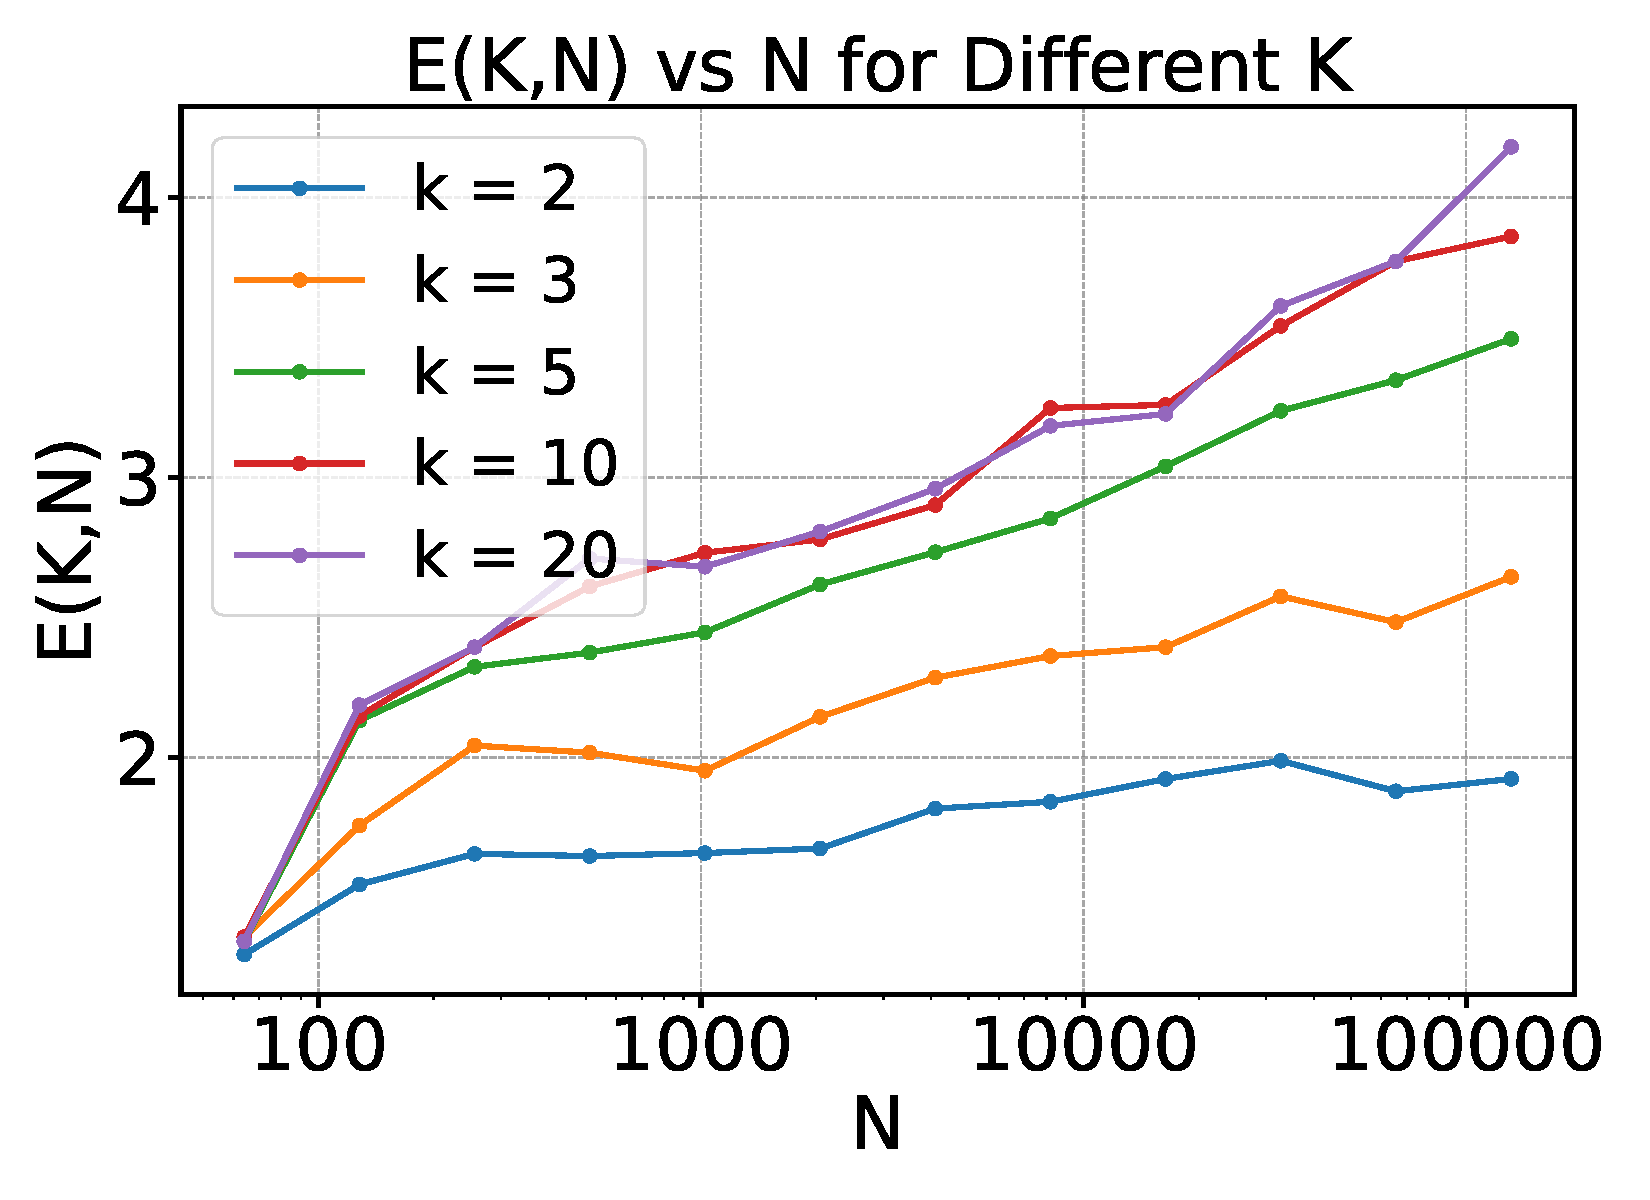
\includegraphics[width=\linewidth]{figs/E_k_avg_vs_N_log_wide_bold.pdf}
%         \caption{Strongly convex case: $E(K,N)$ with $N$}
%         \label{fig:strongly-convex-EK-for-N}
%     \end{subfigure}
%     \begin{subfigure}[t]{0.634\linewidth}
%         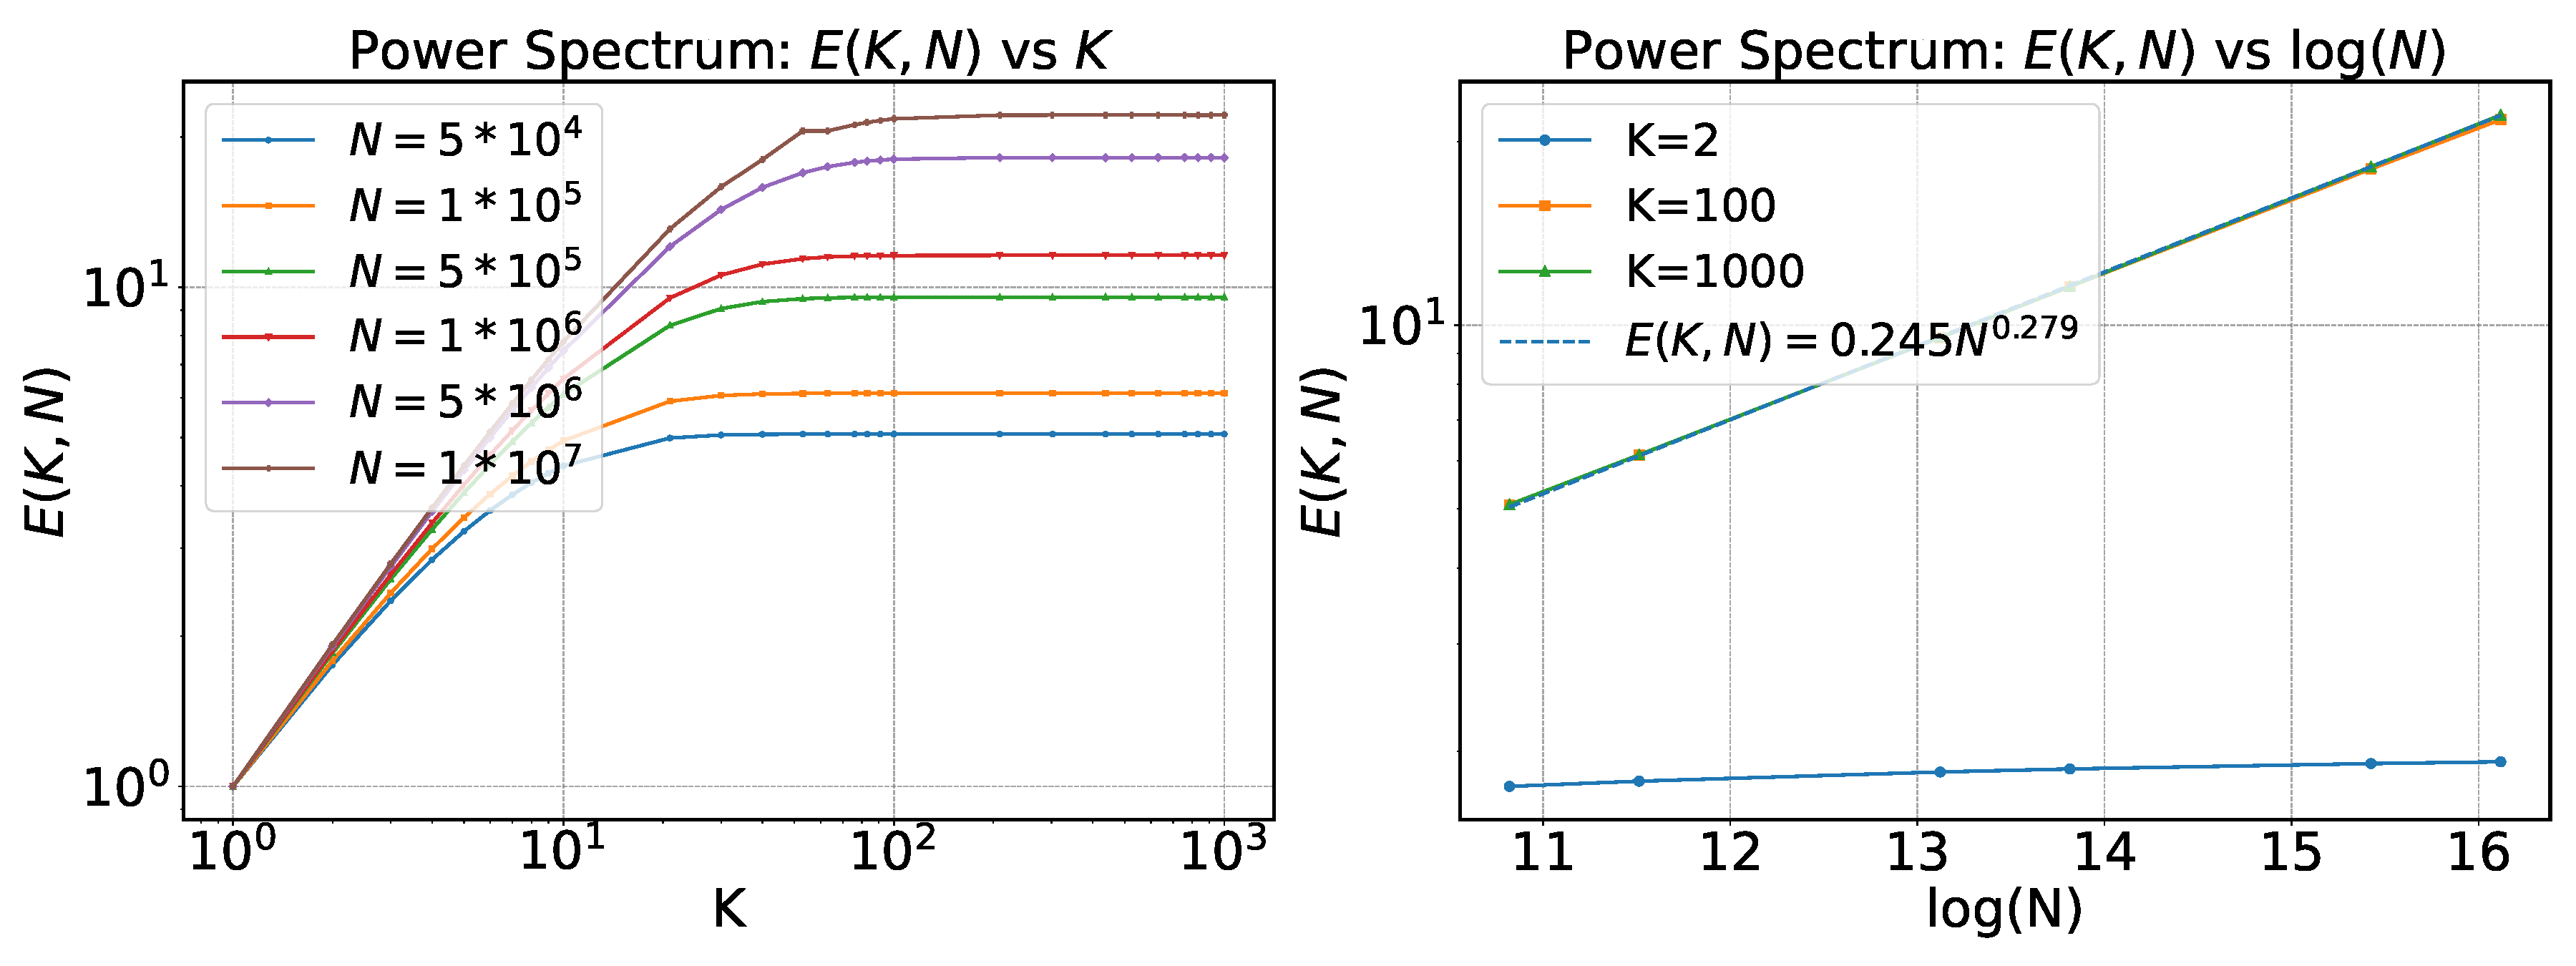
\includegraphics[width=\linewidth]{figs/E_K_comparison_power.pdf}
%         \caption{The solvable cases with power law in simulation.}
%         \label{fig:one-hot}
%     \end{subfigure}
%     \caption{Simulation Experiments.}
%     % \haodong{rewrite the caption, reorganize the subfigures; replot the firgure (a), plot from $N=64$}
%     % \tingkai{strongly-convex + power, put log into the appendix; delete the grid in strongly convex case}
% % \vspace{-0.25in}
% \end{figure}
% \vspace{-0.2in}
\subsection{Empirical Validation on Large Language Models}\label{sec:experiment-llm}

% To examine whether our theoretical predictions on effective reuse rate hold on different large language model training regimes and model sizes, we conduct experiments on two representative large language models: a 0.3B-parameter model trained from scratch and a 1.7B-parameter model fine-tuned on downstream data. The 0.3B pretraining experiment, which provides a direct verification of our theory, is described in the main text. The 1.7B fine-tuning experiment is presented in \Cref{app:metamath_experiment} due to space constraints.
% \vspace{-0.2mm}

% \begin{figure}[htbp]
   % \begin{subfigure}[b]{0.48\linewidth}
    %     \includegraphics[width=\linewidth]{figures/LLM/loss_over_step.pdf}
    %     \caption{Training loss as a function of training steps for different fresh data sizes.}
    %     \label{fig:loss-step}
    % \end{subfigure}
% \begin{figure}[t!]
%     % \vspace{-0.7in}
%     \centering
%     \begin{subfigure}[b]{0.48\linewidth}
%          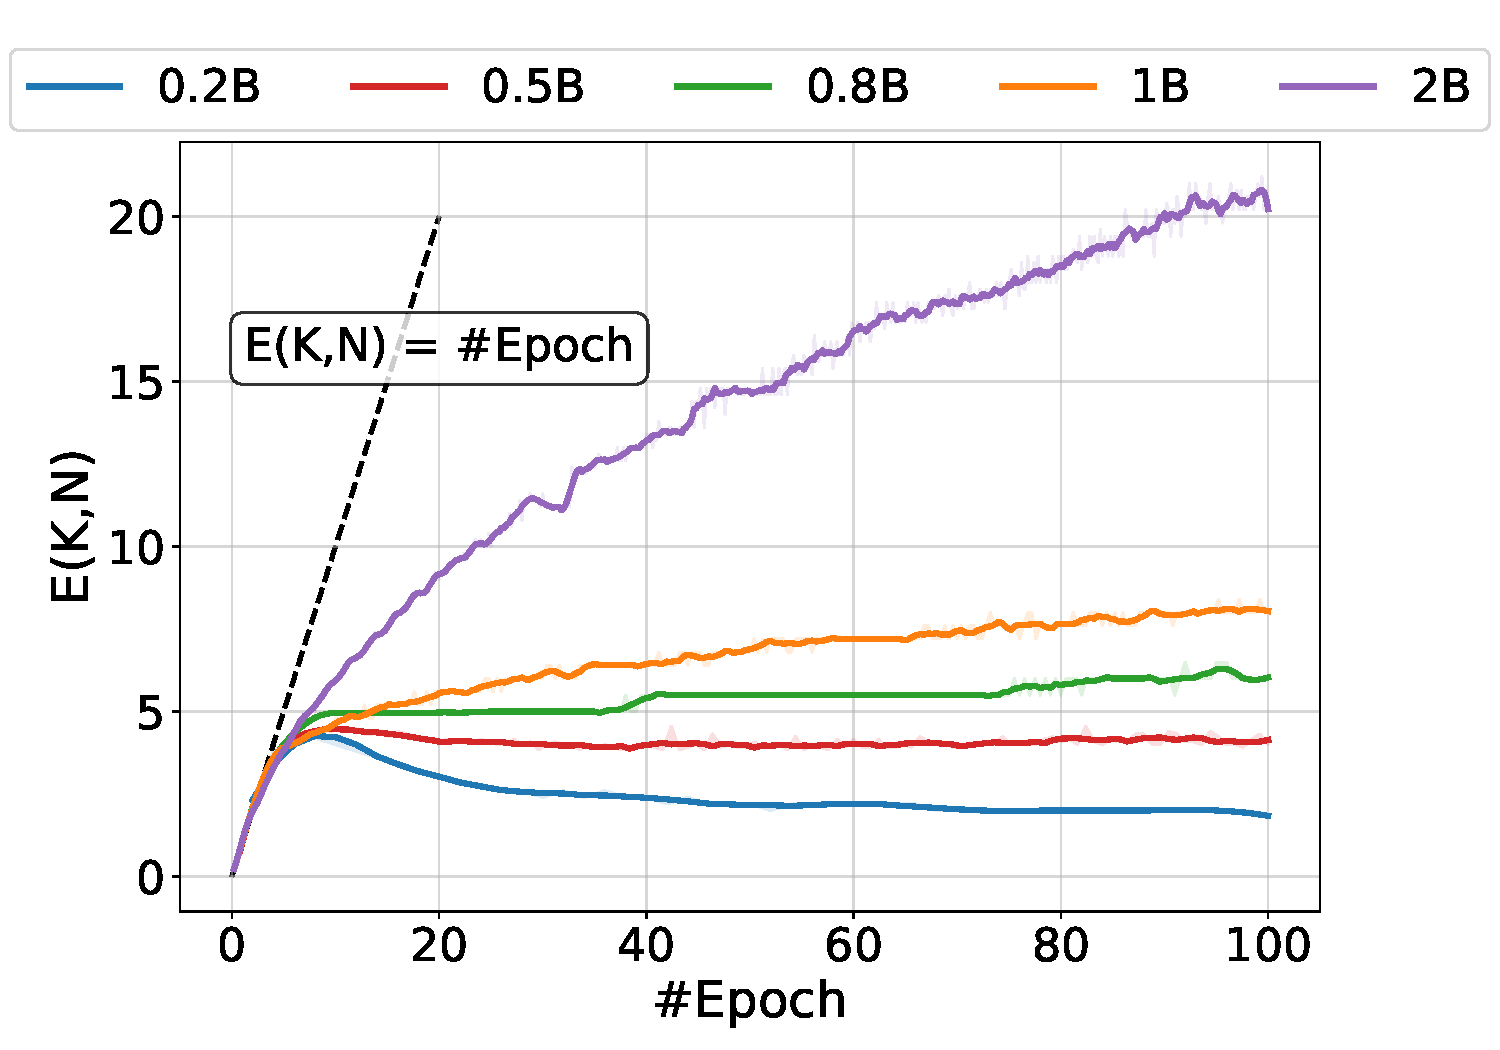
\includegraphics[width=\linewidth]{figs/E_k_smoothed_shaded.pdf}
%          \caption{The effective reuse rate $E(K,N)$ as a function of the epoch number $K$.}
%         % \caption{The effective reuse rate $E(K,N)$ as a function of the number of training epochs $K$ for varying fresh data sizes $N$. The shaded regions represent the variability from the smoothed trend in different epochs.}
%         \label{fig:ek-k}
%     \end{subfigure}   
%     \hfill
%     \begin{subfigure}[b]{0.48\linewidth}
%         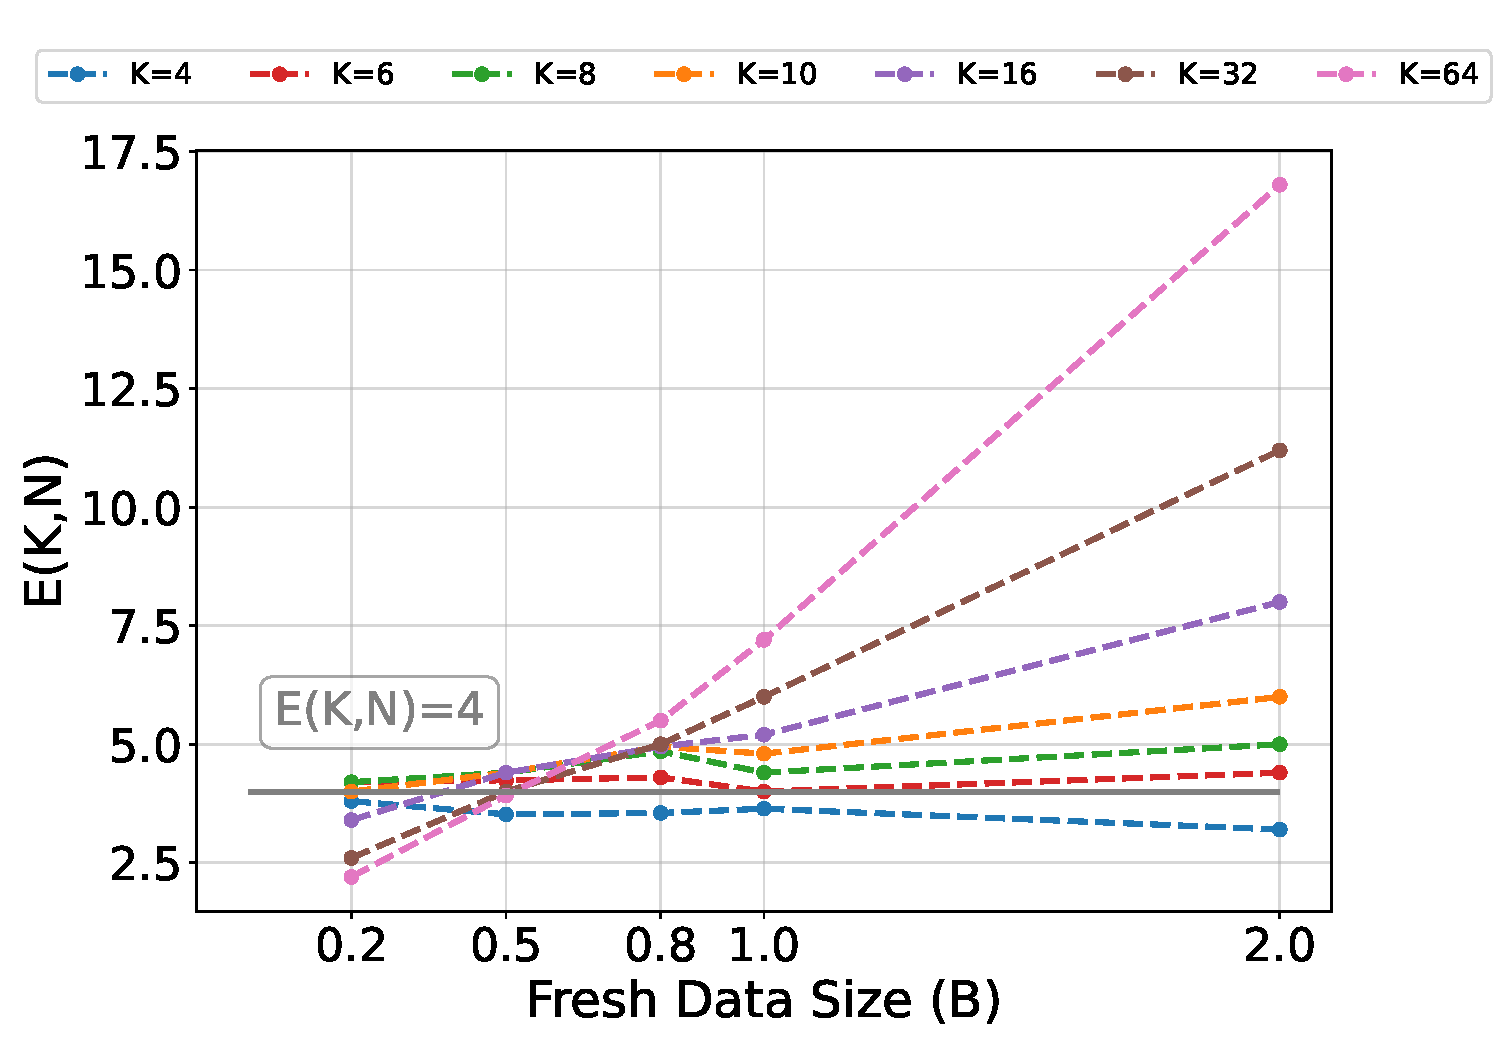
\includegraphics[width=\linewidth]{figs/E_k_over_fresh_data_size.pdf}
%         \caption{The effective reuse rate $E(K,N)$ as a function of the fresh data size $N$.}
%         \label{fig:ek-data}
%     \end{subfigure}
%     \caption{The effective reuse rate $E(K,N)$ over $K$ and $N$ in language model experiments.}
%     % \caption{}
%     % \caption{\textbf{Left:} Training loss progression over training steps. \textbf{Right:} The saturated effective reuse rate $E(K,N)$ in relation to the size of the fresh dataset $N$.}
%     % \vspace{-0.2in}
% \end{figure}

% \begin{figure}[t]
%     % \vspace{-0.4in}
%     \centering
%     \includegraphics[width=0.5\linewidth]{figs/E(K, N) vs N_ws3_ratio0.75_alpha0.9_exp.pdf}
%     \caption{The saturation points $K(\lambda,N)$ as a function of the dataset size N.}
%     \label{fig:ek-n-saturation point}
%     \vspace{-0.2in}
% \end{figure}


\begin{comment}
\begin{figure}[t!]
    \centering
    \subfigure[The effective reuse rate $E(K,N)$ as a function of the epoch number $K$.%
      \label{fig:ek-k}]{
        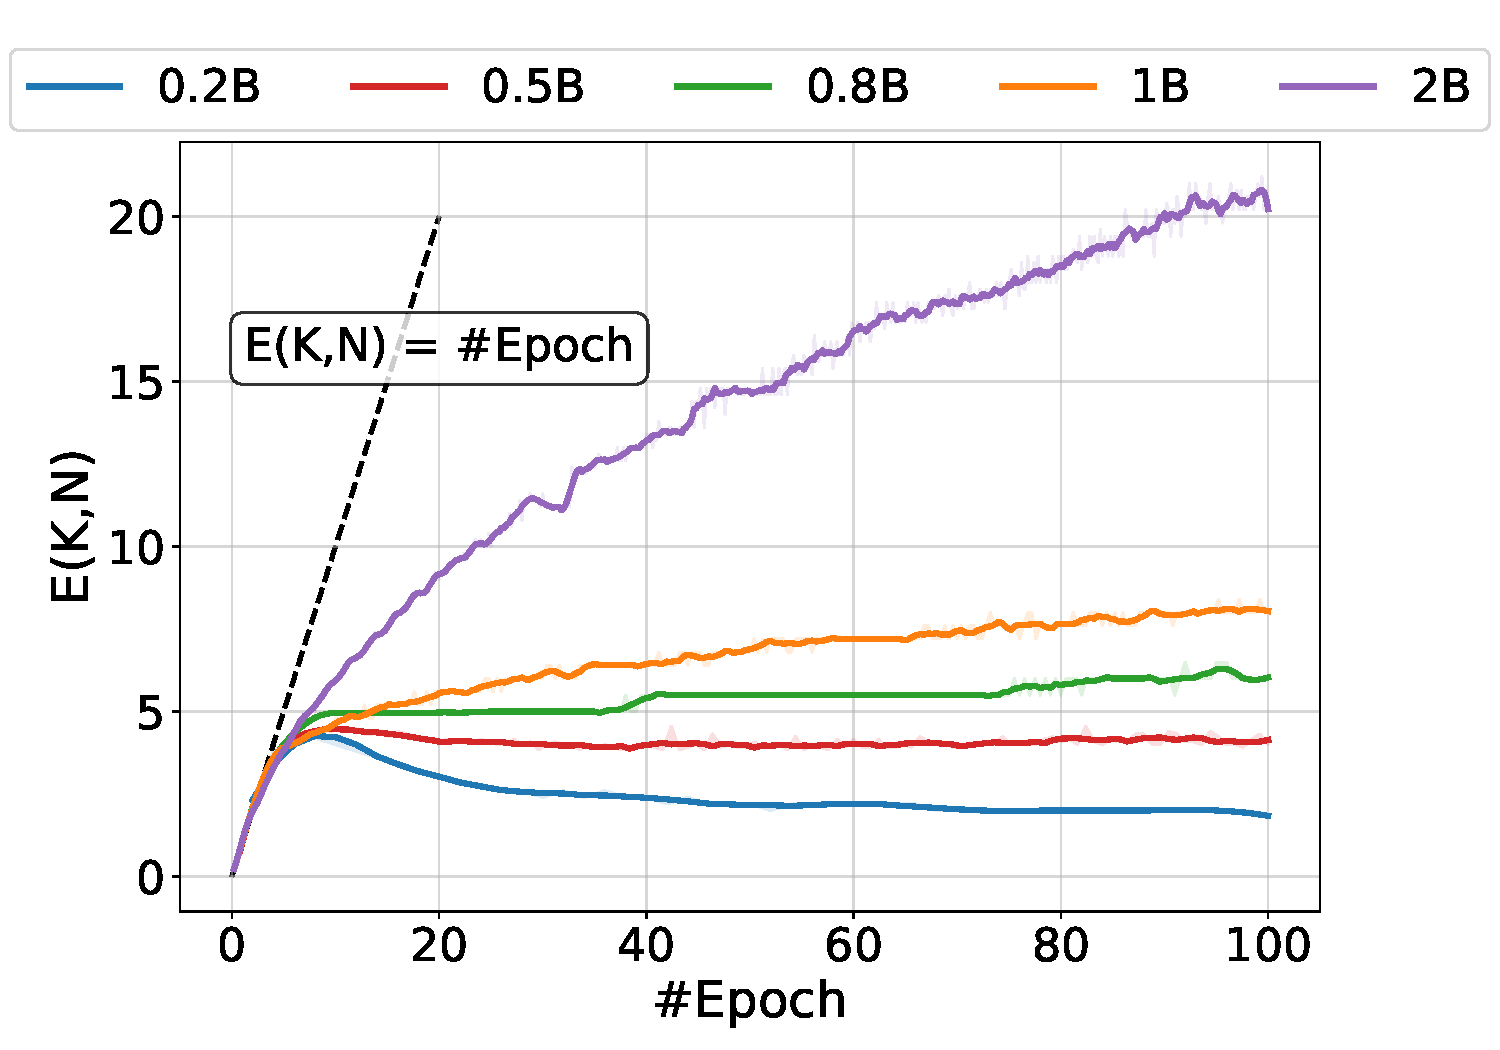
\includegraphics[width=0.48\linewidth]{figs/E_k_smoothed_shaded.pdf}
    }\hfill
    \subfigure[The effective reuse rate $E(K,N)$ as a function of the fresh data size $N$.%
      \label{fig:ek-data}]{
        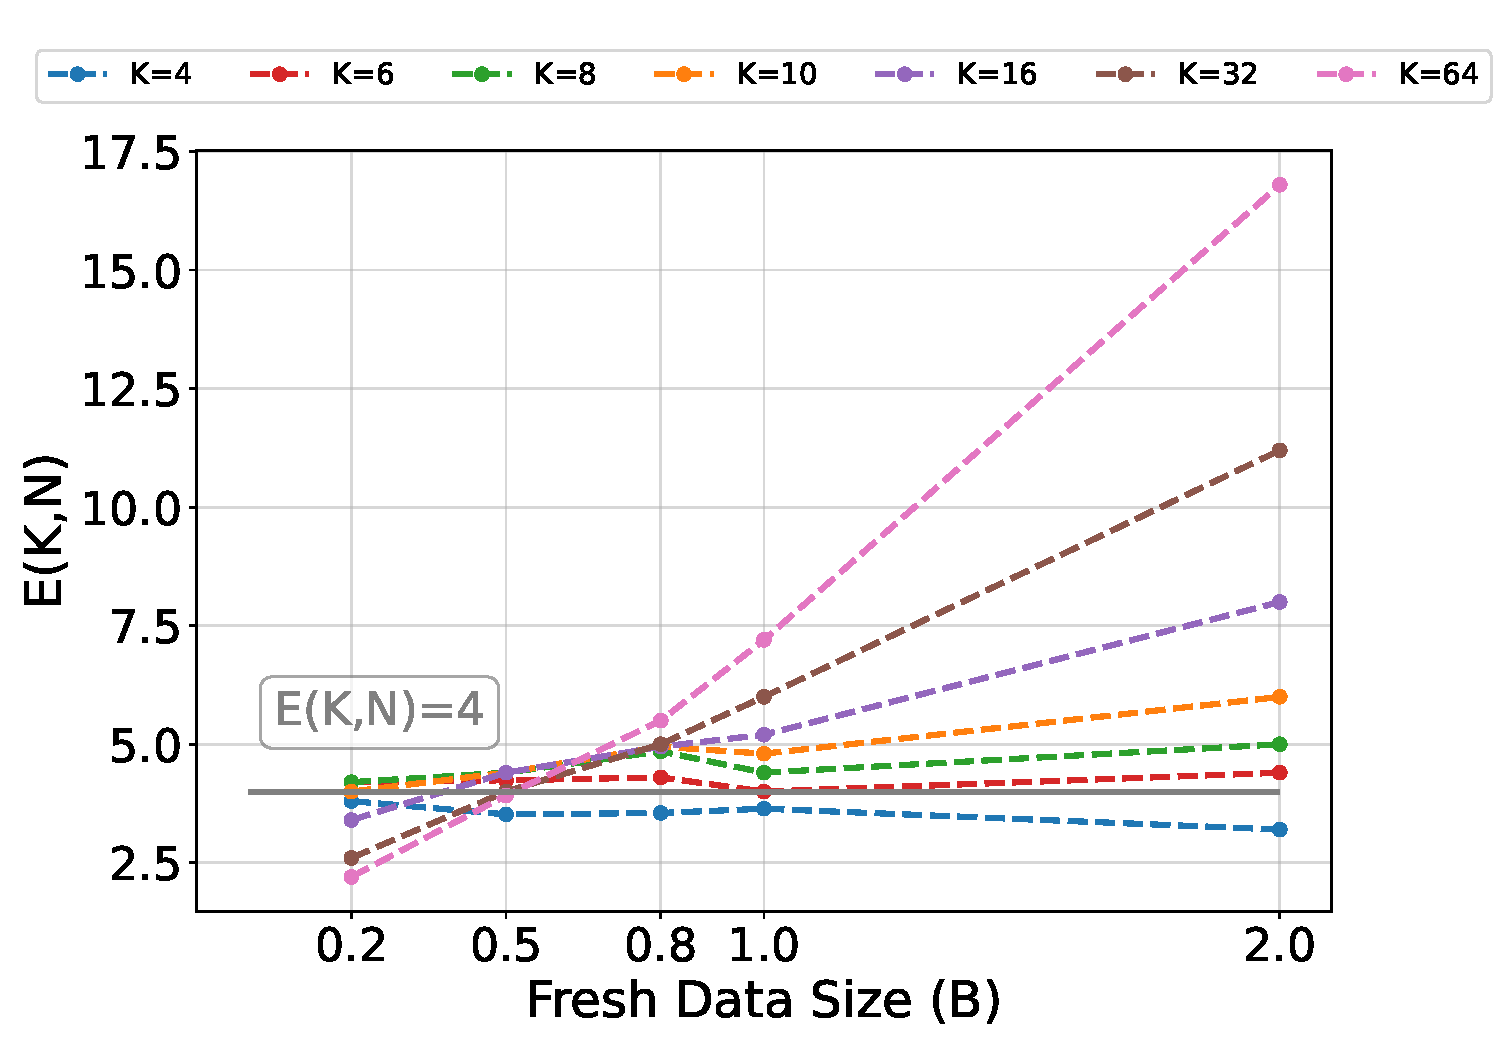
\includegraphics[width=0.48\linewidth]{figs/E_k_over_fresh_data_size.pdf}
    }
    \caption{The effective reuse rate $E(K,N)$ over $K$ and $N$ in language model experiments.}
\end{figure}
\end{comment}


% \paragraph{Experiments Setup.} To empirically validate that larger datasets enable more effective repetition, we pretrained a large language model with fresh data sizes from 0.2B to 2B tokens (100 epochs each), and a 200B-token control. The effective reuse rate, $E(K,N) = N_f(K,N)/N$, was approximated by determining the fresh data size $N_f(K,N)$ for equivalent single-pass validation loss. We used a 0.3B parameter model (adapted from Qwen2.5-0.5B~\citep{qwen2025qwen25technicalreport}), a 200B-token DCLM subset, and a constant learning rate (to align with theory and avoid learning rate effects~\citep{hoffmann2022training,luo2025multi}). See \Cref{app:setup} for details.

% \paragraph{When $K\le 4$, $E(K,N) \approx K$.} Our theory predicts $E(K,N) \approx K$ for small $K$ (e.g., $K\le 4$). \Cref{fig:loss-step} shows that insufficient data (0.2B tokens) leads to overfitting, which is reduced by larger datasets. Consequently, the difference between multi-epoch and single-pass performance decreases. As shown in \Cref{fig:ek-k,fig:ek-data}, $E(K,N)$ increases with $K$ for small $K$ ($\approx K$ for $K\le 5$) and saturates near $K$ at $K=4$, aligning with data-constrained scaling laws~\citep{muennighoff2023scaling}.

% \paragraph{Larger Datasets Allow More Repetition.} $E(K,N)$ increases with epochs and saturates (towards $K$) for sufficiently large datasets, challenging the assumption of a uniform effective number of epochs across dataset sizes in~\citet{muennighoff2023scaling}. \Cref{fig:ek-data} shows $E(K,N)$ increases monotonically with dataset size (before saturating to $K$, as seen for $K\ge 16$). With 2B tokens, $E(K,N)$ continues to grow after 100 epochs (\Cref{fig:ek-k}), implying that repeating 2B tokens 100 times is equivalent to using over 40B fresh tokens, and suggesting further pretraining scaling with larger datasets.

\paragraph{Experiments Setup.} We conduct experiments on a large language model to empirically validate the hypothesis that larger datasets allow for more effective repetition. We perform pretraining runs with fresh data sizes of 0.2B, 0.5B, 0.8B, 1.0B, and 2B tokens, each trained for 100 epochs. As a control, we also include a run with 200B fresh tokens. For each fresh dataset size $N$ and training epoch $K$, we approximate the effective reuse rate $E(K,N)$ by determining the effective fresh data size $N_f(K,N)$ required to achieve the same validation loss after one pass through the data. The effective reuse rate is then computed as: $E(K,N)=\frac{N_f(K,N)}{N}$.
% \label{eq:llm}

Our experiments utilize a 0.3B parameter model adapted from the Qwen2.5-0.5B architecture~\citep{qwen2025qwen25technicalreport} and a subset of the DCLM dataset, totaling 200B tokens.
%The smaller-than-standard model size is chosen due to the substantial computational cost associated with multi-epoch pretraining.
A separate subset of the DCLM dataset is reserved for validation. Crucially, we use a constant learning rate schedule across all experiments to align with our theoretical analysis and mitigate the confounding effects of learning rate schedules, as reported in prior work~\citep{hoffmann2022training,luo2025multi}. ~\Cref{fig:ek-k} depicts the relationship between $E(K,N)$ and $K$. ~\Cref{fig:loss-step} depicts the training curves for different data sizes, and marks the points of different curves where $E(K,N)=\lambda K$, where $\lambda$ controls how strict the criterion is for determining when multi-epoch training begins to underperform one-pass training. Given such $\lambda$, we denote the corresponding number of training epochs as $K(\lambda, N)$, which we refer to as \textit{saturation points}. In our experiments, we take $\lambda = 0.75$. Further, in \Cref{fig:ek-n-saturation point}, we show the precise relationship between $K(\lambda, N)$ and $N$. More details regarding the experiment setup are available in Appendix~\ref{app:setup}.


% These points mark where multi-epoch training begins to underperform compared with single-epoch training. 
% We compute $E(K,N) = \lambda K$ for $11$ uniformly spaced values of $\lambda$ in the range $[0.8,0.9]$ and average the resulting $E(K,N)$ values as the separation point value. Here we use multiple values of $\lambda$ because the curve exhibits randomness, and averaging over several choices yields a more reliable trend. 




% Moreover, model size is also a key factor in real LLM training.
% Furthermore, in Figure~3 we visualize, for each fresh data size $N$, the saturation-point value of $E(K,N)$ at which multi-epoch training first starts to underperform the one-pass baseline. This shows how the recommended effective reuse rate varies with $N$, and we fit these saturation points as a function of $N$ to obtain an empirical rule for choosing the number of passes; see Appendix~C.2 for details of the fitting procedure. To assess the robustness of our conclusions with respect to the learning-rate schedule, we additionally repeat the analysis under a trapezoidal learning-rate schedule; the experimental setup and results are described in Appendix~C.3.


% \begin{figure}[t]
%     % \vspace{-0.4in}
%     \centering
%     \includegraphics[width=0.5\linewidth]{figs/E(K, N) vs N_ws3_ratio0.75_alpha0.9_exp.pdf}
%     \caption{The saturation points $K(\lambda,N)$ as a function of the dataset size N.}
%     \label{fig:ek-n-saturation point}
%     \vspace{-0.2in}
% \end{figure}

\paragraph{Previous Work: When $K\le 4$, $E(K,N) \approx K$.} Our theoretical analysis indicates that $E(K,N)$ should be close to $K$ when $K$ is small (e.g., $K\le 4$). 
% In \Cref{fig:loss-step}, we show the validation losses for different fresh data sizes as they vary with the training steps. When the fresh data is insufficient, such as 0.2B tokens, the training run experiences overfitting, where the validation loss starts to increase as training progresses. As the fresh data size increases, the validation loss decreases at the same training step. Furthermore, the performance difference between multi-epoch training and a single pass through the data becomes smaller with larger fresh datasets. Computing $E(K, N)$, we present the variation of $E(K, N)$ with both $K$ and $N$ in~\Cref{fig:ek-k,fig:ek-data}.
In Figure~\ref{fig:ek-k}, when the epoch number is small (approximately $\le 5$), we observe that $E(K,N)$ increases at a rate comparable to the epoch number, 
as indicated by the black dashed line. 
% Moreover, in the case of $K=4$, $E(K,N)$ saturates close to $K$ across different fresh data sizes, as depicted by the blue line and gray baseline in~\Cref{fig:ek-data}. 
Thus our predictions of $E(K,N)$ when $K$ is small aligns with the data-constrained scaling laws~\citep{muennighoff2023scaling}. 

\paragraph{Larger Datasets Allow More Repetition.}
$E(K,N)$ increases with the number of fresh data sizes and eventually saturates 
% (towards $K$) 
for sufficiently large fresh datasets. Our results challenge the data-constrained scaling laws proposed by~\citet{muennighoff2023scaling}, which assume a uniform effective number of epochs across different fresh data sizes. In Figure~\ref{fig:loss-step}, we show that at the critical points where one-pass training start to outperform multi-epoch training significantly, $E(K,N)$ increases as $N$ increases. This suggests the continued potential for scaling pretraining through multi-epoch training with larger datasets.


% \haodong{replace tuning point with saturation point or Separation point, anyway, give it a clear definition}
\paragraph{Fitting Experiments.}In \Cref{fig:ek-n-saturation point}, to provide real-world evidence that larger datasets can be repeated more, we plot the saturation point values for different $N$ to illustrate how they vary with $N$. Then we fit them as a function of $N$; see Appendix~\ref{app:fitting experiments} for details of the fitting procedure. 

% Further, we show the precise relationship between the saturation points and $N$ in \Cref{fig:ek-n-saturation point}. 
Surprisingly, though we do not claim that $E(K,N) = \Theta(\log N)$ holds for general LLM trainings when $K$ is large, as we calculated in the strongly convex linear regression case, here we do observe that $K(\lambda,N)$ gradually increases when $N$ increases, and it follows that $K(\lambda,N) \approx 0.80 \log N + 5.21$ with the correlation coefficient being $r = 0.97$. In this formula, the dataset $N$ is measured in billions of tokens (B).

\paragraph{Experiments with Learning Rate Decay.}For further investigation of the scaling behaviour of multi-epoch training, we conduct LLM experiments with a non-constant learning rate schedule, aligning with the common practice in reality. Specifically, we additionally repeat the above analysis with a WSD learning rate schedule with linear decay. The experimental setup and results are described in Appendix~\ref{app:experiment-llm-lrs}.

% \paragraph{Limitations of LLM experiments.} 


% characterizes this relationship precisely, namely $E(K,N) = \Theta\left(\log N\right)$, with the correlation coefficient of the fit being $r=0.99$.
% In contrast, as clearly presented in \Cref{fig:ek-data}, for the same epoch number, $E(K,N)$ values monotonically increase with the fresh data size before $E(K,N)$ saturates to $K$, as seen in cases with $K\ge 16$ in our experiment. Furthermore, except in the insufficient fresh data scenario (before saturation), the effective reuse rate monotonically increases as the epoch number increases. Remarkably, even after 100 repetitions with a large fresh dataset size (2B tokens in our experiment), the effective number of epochs has not yet converged, as shown in~\Cref{fig:ek-k}. Specifically, repeating 2B data for 100 epochs is equivalent to over 40B fresh data based on validation loss. 


% \kairong{Align notations with theory part.}
% \paragraph{Experiments Setup.} We conduct experiments on a large language model to empirically validate the hypothesis that larger datasets allow for more effective repetition. We perform pretraining runs with fresh data sizes of 0.2B, 0.5B, 0.8B, 1.0B, and 2B tokens, each trained for 100 epochs. As a control, we also include a run with 200B fresh tokens. For each fresh dataset size $N$ and training epoch $K$, we approximate the effective reuse rate $E(K,N)$ by determining the effective fresh data size $N_f(K,N)$ required to achieve the same validation loss after one pass through the data. The effective reuse rate is then computed as:
% \begin{equation}\label{eq:llm}
%     E(K,N)=\frac{N_f(K,N)}{N}.
% \end{equation}
% Our experiments utilize a 0.3B parameter model adapted from the Qwen2.5-0.5B architecture~\citep{qwen2025qwen25technicalreport} and a subset of the DCLM dataset, totaling 200B tokens. The smaller-than-standard model size is chosen due to the substantial computational cost associated with multi-epoch pretraining. A separate subset of the DCLM dataset is reserved for validation. Crucially, we use a constant learning rate schedule across all experiments to align with our theoretical analysis and mitigate the confounding effects of learning rate schedules, as reported in prior work~\citep{hoffmann2022training,luo2025multi}. See~\Cref{app:setup} for more details for experiment setup.

% \paragraph{When $K\le 4$, $E(K,N)=K$.} Our theoretical analysis indicates $E(K,N)$ should close to $K$ when $K$ is small (e.g., $K\le 4$). In \Cref{fig:loss-step}, we show the validation losses of different fresh data sizes, vary with the training steps. When the fresh data is too insufficient, like 0.2B token, the training run is trapped by overfitting, where the validation loss begins to increase as training progresses. As the fresh data size increases, the validation loss goes lower at the same training step. Furthermore, the performance gap between multi-epoch training and a single pass through the data diminishes with larger fresh datasets. Computing $E(K, N)$ by~\Cref{eq:llm}, we conclude in~\Cref{fig:ek-k,fig:ek-data} to exhibit the variation of $E(K, N)$ along both $K$ and $N$. In~\Cref{fig:ek-k}, when the epoch number is small (approximately $\le 5$), we find $E(K,N)$ increases at a comparable rate with the epoch number, which is captured by the pink dash line. What's more, in the case of $K=4$, $E(K,N)$ saturate close to $K$ across different fresh data sizes, as dipicted by the blue line and gray baseline in~\Cref{fig:ek-data}. The fresh-data equivalent repetition for modest multi-epoch pretraining, aligns with the data-constrained scaling laws~\citep{muennighoff2023scaling}.

% \paragraph{Larger Datasets can be Repeated More.}
% $E(K,N)$ increases with the number of training epochs and eventually saturates (to $K$) for sufficiently large fresh datasets. Our results challenge the data-constrained scaling laws in prior~\citet{muennighoff2023scaling}, who assumed a uniform effective number of epochs across different fresh data sizes. On the contrary, as clearly presented in \Cref{fig:ek-data}, given the same epoch number, $E(K,N)$ values monotonically increase with the fresh data size, before $E(K,N)$ saturates to $K$, like cases $K\ge 16$ in our experiment. And except the insufficient fresh data scenario (before saturated), the effective reuse rate monotonically increases as the epoch number increases. Remarkably, even after 100 repetitions with a large fresh dataset size (2B tokens in our experiment), the effective number of epochs has not yet converged as shown in~\Cref{fig:ek-k}. Specifically, repeating 2B data for 100 epochs is equivelent to over 40B fresh data using the measurement of validation loss. This suggests the continued potential for scaling pretraining through multi-epoch training with larger datasets.


% \paragraph{Experiments Setup.} We conduct experiments on a large language model to empirically validate the hypothesis that larger datasets allow for more effective repetition. We perform pretraining runs with fresh data sizes of 0.2B, 0.5B, 0.8B, 1.0B, and 2B tokens, each trained for 100 epochs. As a control, we also include a run with 200B fresh tokens. For each fresh dataset size $N$ and training epoch $K$, we approximate the effective reuse rate $E(K,N)$ by determining the effective fresh data size $N_f(K,N)$ required to achieve the same validation loss after one pass through the data. The effective reuse rate is then computed as: $E(K,N)=\frac{N_f(K,N)}{N}$.
% % \label{eq:llm}

% Our experiments utilize a 0.3B parameter model adapted from the Qwen2.5-0.5B architecture~\citep{qwen2025qwen25technicalreport} and a subset of the DCLM dataset, totaling 200B tokens.
% %The smaller-than-standard model size is chosen due to the substantial computational cost associated with multi-epoch pretraining.
% A separate subset of the DCLM dataset is reserved for validation. Crucially, we use a constant learning rate schedule across all experiments to align with our theoretical analysis and mitigate the confounding effects of learning rate schedules, as reported in prior work~\citep{hoffmann2022training,luo2025multi}. More details regarding the experiment setup are available in~\Cref{app:setup}.

% \paragraph{When $K\le 4$, $E(K,N) \approx K$.} Our theoretical analysis indicates that $E(K,N)$ should be close to $K$ when $K$ is small (e.g., $K\le 4$). In \Cref{fig:loss-step}, we show the validation losses for different fresh data sizes as they vary with the training steps. When the fresh data is insufficient, such as 0.2B tokens, the training run experiences overfitting, where the validation loss starts to increase as training progresses. As the fresh data size increases, the validation loss decreases at the same training step. Furthermore, the performance difference between multi-epoch training and a single pass through the data becomes smaller with larger fresh datasets. Computing $E(K, N)$, we present the variation of $E(K, N)$ with both $K$ and $N$ in~\Cref{fig:ek-k,fig:ek-data}. In~\Cref{fig:ek-k}, when the epoch number is small (approximately $\le 5$), we observe that $E(K,N)$ increases at a rate comparable to the epoch number, as indicated by the pink dashed line. Moreover, in the case of $K=4$, $E(K,N)$ saturates close to $K$ across different fresh data sizes, as depicted by the blue line and gray baseline in~\Cref{fig:ek-data}. The fresh-data equivalent repetition for modest multi-epoch pretraining aligns with the data-constrained scaling laws~\citep{muennighoff2023scaling}.

% \paragraph{Larger Datasets Allow More Repetition.}
% $E(K,N)$ increases with the number of training epochs and eventually saturates (towards $K$) for sufficiently large fresh datasets. Our results challenge the data-constrained scaling laws proposed by~\citet{muennighoff2023scaling}, who assumed a uniform effective number of epochs across different fresh data sizes. In contrast, as clearly presented in \Cref{fig:ek-data}, for the same epoch number, $E(K,N)$ values monotonically increase with the fresh data size before $E(K,N)$ saturates to $K$, as seen in cases with $K\ge 16$ in our experiment. Furthermore, except in the insufficient fresh data scenario (before saturation), the effective reuse rate monotonically increases as the epoch number increases. Remarkably, even after 100 repetitions with a large fresh dataset size (2B tokens in our experiment), the effective number of epochs has not yet converged, as shown in~\Cref{fig:ek-k}. Specifically, repeating 2B data for 100 epochs is equivalent to over 40B fresh data based on validation loss. This suggests the continued potential for scaling pretraining through multi-epoch training with larger datasets.